\begin{savequote}[75mm]
The real voyage of discovery consists not in seeking new landscapes, but in having new eyes.
\qauthor{Marcel Proust}
\end{savequote}

\chapter{The discovery of the Higgs boson and the role of the $H\rightarrow WW^{*}\rightarrow \ell\nu\ell\nu$ channel}

\section{Introduction}

This chapter presents the results of the search for the Higgs boson in $4.8 \ifb$ collected at $\sqrt{s} = 7 \TeV$ and $5.8 \ifb$ at $\sqrt{s} = 8 \TeV$. The results of three searches at $\sqrt{s} = 8 \TeV$ in the \HWWfull, $H\to \gamma \gamma$, and $H\to ZZ \to 4\ell$ channels are shown. These results at $8 \TeV$ are combined with the results of searches at $\sqrt{s} = 7 \TeV$ in the same channels along with $H\to\tau\tau$ production and associated production searches for $H\to b\bar{b}$. The results of this combination are a $5.9 \sigma$ detection of a new particle consistent with a Higgs boson produced via gluon fusion. Rather than going into detail for all of the different Higgs decay searches, this chapter will discuss the three most sensitive channels and in particular focus on \HWWfull, the topic of this thesis. While the focus is on $WW^*$, some of the $ZZ^*$ and $\gamma\gamma$ results are shown for completeness. The results not discussed here can be found in the ATLAS Higgs discovery publication~\cite{Discovery}.


\section{Data and simulation samples}

The data sample used for the following results was taken in 2011 and 2012 at center of mass energies of $7$ and $8 \TeV$, respectively, with $4.8 \ifb$ collected at $7 \TeV$ and $5.8 \ifb$ collected at $8 \TeV$. Higgs production in the gluon fusion and vector boson fusion modes is modeled with \POWHEG for the hard scattering event and \PYTHIA for the showing and hadronization. Associated production of a Higgs with a vector boson or top quarks is modeled via \PYTHIA. Table~\ref{tab:disc_mc} shows the Monte Carlo generators used for modeling the signal and background processes relevant for the three analyses to be discussed. 

\begin{table}[h!]
\centering
\captionsetup{justification=centering}

%\begin{tabular*}{0.480\textwidth}{p{0.075\textwidth} p{0.180\textwidth} l}
\hspace{-10pt}
\begin{tabular}{cc}
\dbline
Process & Generator \\ \hline
ggF, VBF $H$ & \POWHEG + \PYTHIA \\ 
$WH$, $ZH$, $t\bar{t}H$ & \PYTHIA \\ \hline
$W$+jets, $\ZDY$ + jets & \ALPGEN + \HERWIG \\ 
$t\bar{t}$, $tW$, $tb$ & \MCATNLO + \HERWIG \\ 
$tqb$ & \ACERMC + \PYTHIA \\ 
$q\bar{q} \to WW$ & \MCATNLO + \HERWIG \\ 
$gg \to WW$ & \GGTOWW + \HERWIG \\ 
$q\bar{q} \to ZZ$ & \POWHEG + \PYTHIA \\ 
$gg \to ZZ$ & \GGTOZZ + \HERWIG \\ 
$WZ$ & \MADGRAPH + \PYTHIA, \HERWIG \\ 
$W\gamma$ + jets & \ALPGEN + \HERWIG \\ 
$W\gamma^*$ & \MADGRAPH + \PYTHIA \\ 
$q\bar{q}/gg \to \gamma \gamma$ & \SHERPA \\ \dbline

\end{tabular}

\caption{
Monte Carlo generators used to model signal and background for the Higgs search~\cite{Discovery}.
}
\label{tab:disc_mc}
\end{table} 

\section{$H\to WW \to e\nu\mu\nu$ search}

As discussed in chapter 3, the $H\to WW \to e\nu\mu\nu$ search is unique compared to the $ZZ$ and $\gamma\gamma$ channels. The Higgs mass cannot be fully reconstructed due to the presence of neutrinos in the final state, so the transverse mass $\mT$ is used as the final discriminating variable. This channel also has a wider variety of backgrounds compared to other channels. The same flavor final states are excluded from the $8 \TeV$ dataset due to high pileup conditions\footnote{The less sensitive $7 \TeV$ search result includes both different flavor and same flavor final states.}. These final states were later included in results with the full Run 1 dataset, as discussed in chapters 5 and 6.  

\subsection{Event selection}

The analysis requires two opposite charge isolated leptons, with the leading (sub-leading) lepton required to have $\pT > 25 (15) \GeV$. The events are separated into different signal regions depending on which flavor of lepton is leading ($e\mu$ for leading electron, $\mu e$ for leading muon). Strict lepton quality cuts are applied to the sample to reduce backgrounds from mis-reconstructed leptons.

Jets are reconstructed with the anti-$k_{T}$ algorithm with a radius parameter $R = 0.4$. The jets are required to have $\pT > 25 \GeV$ and $|\eta| < 4.5$, with jets in the tracking volume required to have a jet vertex fraction of $0.5$ and jets in the forward region required to have $\pT > 30 \GeV$. The analysis is separated into three different signal regions based on jet multiplicity: $\Njet = 0, 1, \geq 2$. 

To indicate the presence of neutrinos in the event, a requirement of $\METrel > 25 \GeV$ is made\footnote{For the definition of $\METrel$, see section~\ref{sec:HWW_presel}.}. This requirement significantly reduces the QCD multijet and $\ZDY$ + jets backgrounds. Figure~\ref{fig:disc_njet} shows the distribution of $\Njet$ in data and simulation after applying these ``pre-selection" requirements. 

\begin{figure}[h!]
  %\vspace{20pt}
  \centering
  \captionsetup{justification=centering}
  %\hspace*{-32pt}
  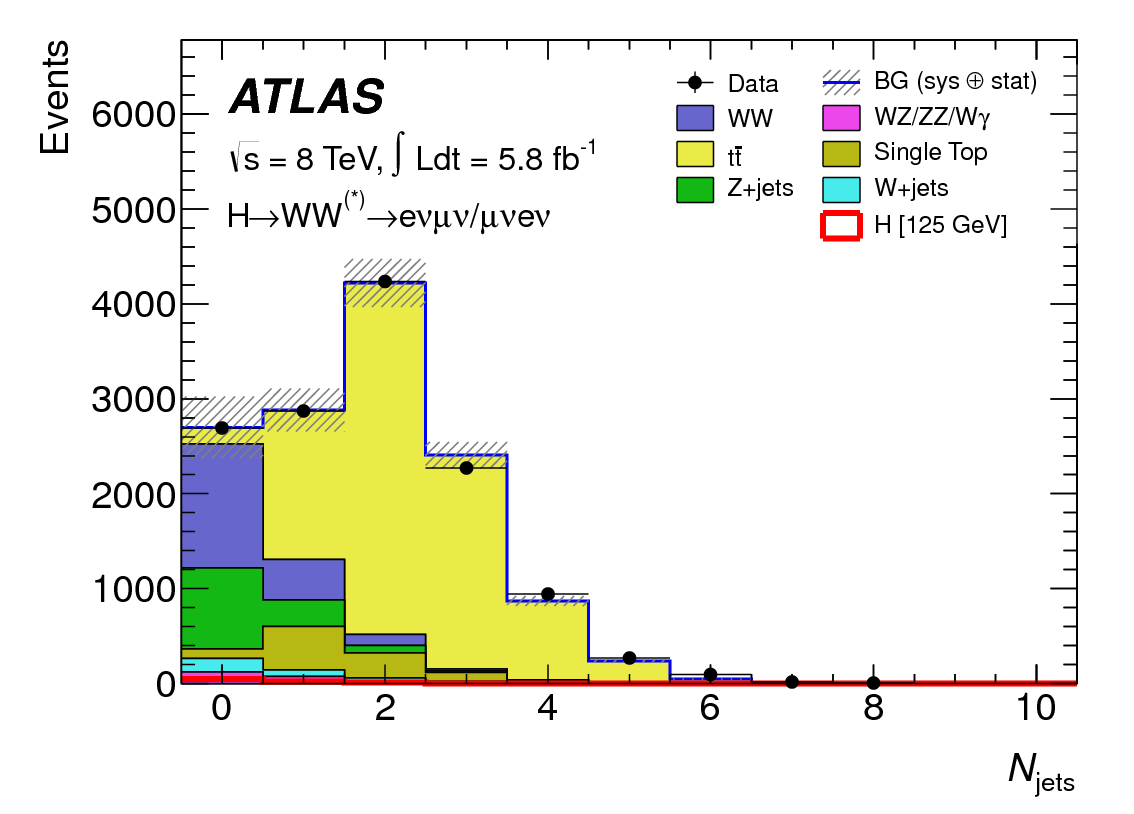
\includegraphics[width=0.6\textwidth]{figures/disc_njet}
  \caption{Jet multiplicity distribution in data and MC after applying lepton, jet, and $\METrel$ selections. The $WW$ and top backgrounds have been normalized using control samples, and the hashed band indicates the total uncertainty on the prediction~\cite{Discovery}.}
  \label{fig:disc_njet}
\end{figure}

Additional selections are applied to require the dilepton topology to correspond to that of a Standard Model Higgs boson. The requirements are presented here - more detailed discussion on the motivation for each requirement can be found in section~\ref{sec:lepton_corr}. In all of the jet multiplicity channels, the dilepton system is required to have a small gap in azimuthal angle, $\dphill < 1.8$. Similarly, the dilepton invariant mass, $\mll$, is required to be less than $50 \GeV$ in the lower jet multiplicity channels and less than $80 \GeV$ in the $\Njet \geq 2$ channel.  In the $\Njet = 0$ channel, the magnitude of the dilepton $\pT$, $\pTll$, is required to be greater than $30 \GeV$. 

In the higher jet multiplicity channels ($\Njet \geq 1$), the top background is a larger fraction of the total background and must be reduced more carefully. The magnitude of the vectorial sum of the $\MET$ with the $\pT$ of the leptons and jets, also known as $\pTtot$, is thus required to be less than $30 \GeV$. Additionally, the di-$\tau$ invariant mass $m_{\tau\tau}$ (dilepton mass computed under the assumption that the neutrinos from the $\tau$ decay are emitted collinear to the charged leptons~\cite{collinear}) is used to reject $Z\to\tau\tau$ events by requiring $|m_{\tau\tau} - m_{Z}| > 25 \GeV$.  

In the $\Njet \geq 2$ channel, requirements are made to isolate the VBF contribution to Higgs production. The kinematics of the two leading jets are used to make these requirements. In particular, the event must have $\dyjj > 3.8$ and $\mjj > 500 \GeV$, along with a veto on having any additional jets with rapidity between the to leading jets. This channel contributed little to the Higgs discovery but became important with the full dataset. This updated analysis is discussed in depth in chapter 5. 

The final discriminating variable used to distinguish the presence of the Higgs signal is the transverse mass, $\mTH$. As discussed in chapter 3, this variable acts as a substitute for the true invariant mass of the Higgs in final states with neutrinos. 

\subsection{Background estimation}

The details of the background estimation techniques used in the \HWWfull analysis are discussed with the full Run 1 dataset in section~\ref{sec:HWWbkg}. The dominant backgrounds are SM $WW$ production and top (both pair and single) production, and these backgrounds have their normalizations estimated from dedicated control regions while their shapes are taken from simulation. 

The control sample for the Standard Model $WW$ background is defined by making the same requirements as the signal region with the $\mll$ requirement inverted (now requiring $\mll > 80 \GeV$) and removing the $\dphill$ requirement. This creates a control sample that is $70$\% ($40$\%) pure in the $0$($1$)-jet region. The correction to the pure MC-based background estimate is quantified by defining a normalization factor $\beta$ which is the ratio of the data yield to the MC yield ($N_{\rm data}/N_{\rm MC}$) in this control sample. Table~\ref{tab:disc_NF} shows the $WW$ normalization factors in the $\Njet = 0$ and $\Njet = 1$ bins (the $\Njet \geq 2$ estimate is taken directly from MC). 

\begin{table}[h!]
\centering
\captionsetup{justification=centering}

%\begin{tabular*}{0.480\textwidth}{p{0.075\textwidth} p{0.180\textwidth} l}
\hspace{-10pt}
\begin{tabular}{|c|c|c|}
\hline
$\Njet$ & $\beta_{WW}$ & $\beta_{t}$ \\ \hline
$ = 0$ & $1.06 \pm 0.06$ & $1.11 \pm 0.06$ \\ \hline
$= 1$ & $0.99 \pm 0.15$ & $1.11 \pm 0.05$  \\ \hline
$\geq 2$ & - & $1.01 \pm 0.26$ \\ \hline
\end{tabular}

\caption{
Normalization factors (ratio of data and MC yields in a control sample) for the Standard Model $WW$ and top backgrounds in the \HWWfull analysis~\cite{Discovery}. Only statistical uncertainties are shown. 
}
\label{tab:disc_NF}
\end{table}

The top background estimate is also computed separately in each jet multiplicity bin. In the $\Njet = 0$ channel, the background is first normalized using data after pre-selection requirements with no selection on $\Njet$. Then, a dedicated $b$-tagged control sample is used to evaluate the ratio of one-jet to two-jet events in data. The details of this technique are shown in reference~\cite{Higgs2011}. In the $\Njet = 1$ and the $\Njet \geq 2$ regions, the top background is normalized in a control sample where the signal region selections are applied, but the $b$-jet veto is reversed and the Higgs topology requirements on $\mll$ and $\dphill$ are removed. The resulting normalization factors for these techniques are shown in table~\ref{tab:disc_NF}. 

\begin{figure}[h!]
  %\vspace{20pt}
  \centering
  \captionsetup{justification=centering}

   \begin{subfigure}[t]{0.5\textwidth}
        \centering
        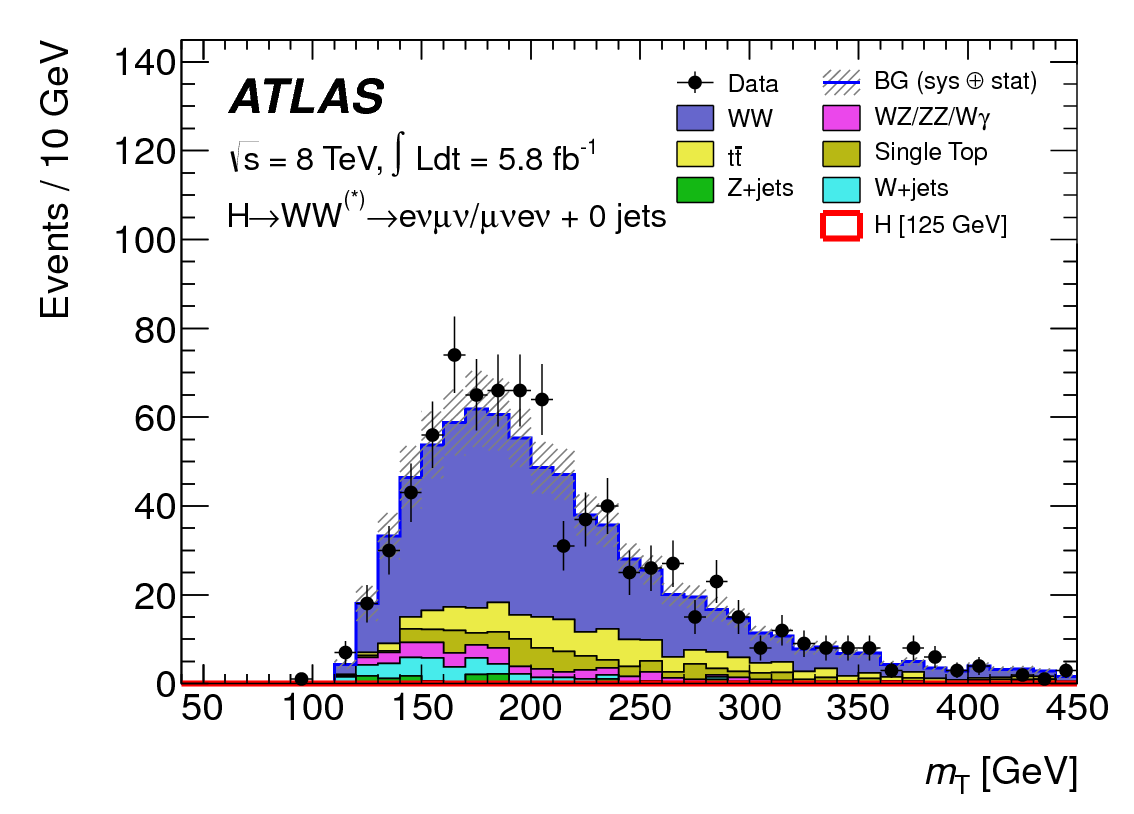
\includegraphics[width=\textwidth]{figures/disc_mt_wwcr}
        \caption{}
    \end{subfigure}%
    \begin{subfigure}[t]{0.5\textwidth}
        \centering
        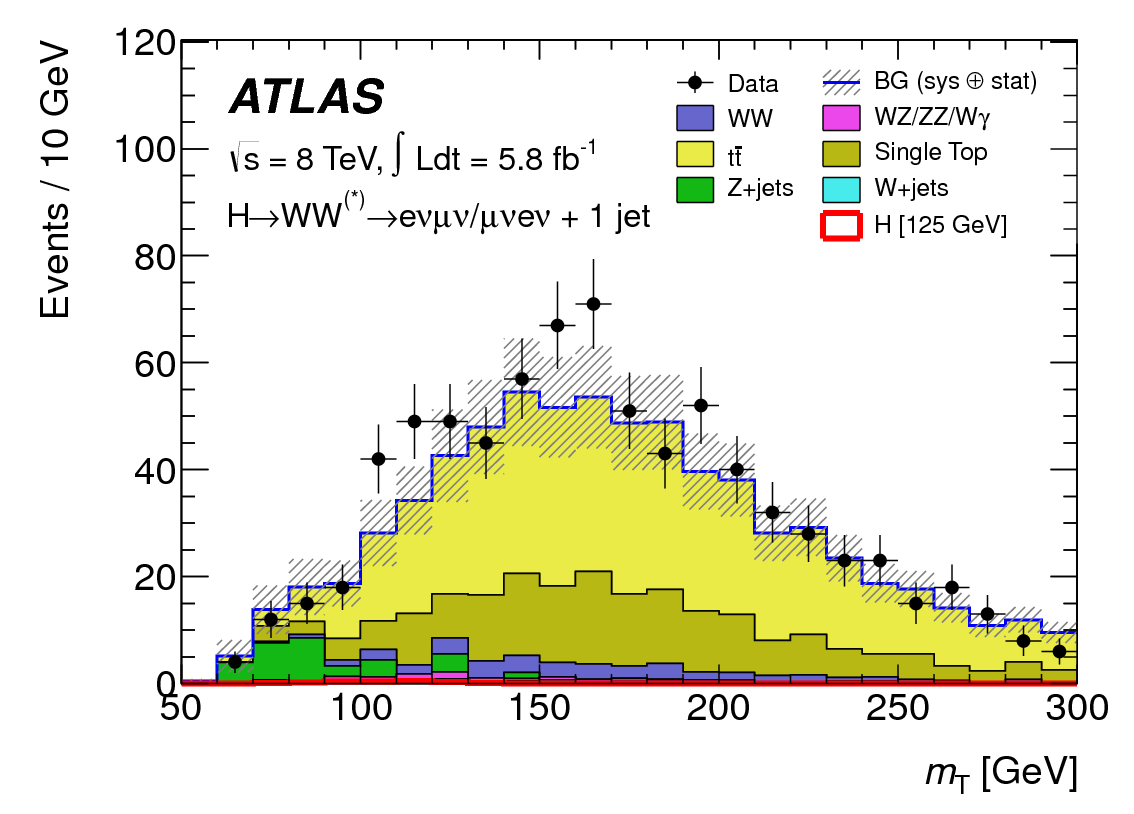
\includegraphics[width=\textwidth]{figures/disc_mt_topcr}
        \caption{}
    \end{subfigure}


   \caption{Comparison of $\mTH$ between data and simulation in the $\Njet = 0$ $WW$ (a) and $\Njet = 1$ top (b) control samples~\cite{Discovery}.}
  \label{fig:disc_mt_cr}
\end{figure}

The control samples which are used for background normalization can also be used to validate the modeling of the $\mTH$ distribution for each background. Figure~\ref{fig:disc_mt_cr} shows the comparison between data and MC for the $\mTH$ distribution after correcting the normalization of the backgrounds in the $WW$ and top control regions. Good agreement between data and simulation is seen in both cases. 

The $W$+jets background estimate is taken entirely from data using a control sample with one well reconstructed lepton and one anti-identified lepton. All other backgrounds are taken purely from simulation. 

\subsection{Systematic uncertainties}

The systematic uncertainties that have the largest impact on the analysis are the theoretical uncertainties associated with the signal cross section, which are shared with the $ZZ^*$ and $\gamma\gamma$ channels. The uncertainties resulting from variations of the QCD scale are $+7\%/-8\%$ on the final signal yield. Those coming from variations of the parton distribution function (PDF) used in the simulation add a $\pm 8\%$ uncertainty on the yield. The uncertainties on the branching ratios of the Higgs are $\pm 5\%$. 

The main experimental uncertainties come from variations of the jet energy scale (JES), jet energy resolution (JER), pile-up, $\MET$, $b$-tagging efficiency, $W$+jets background estimate, and integrated luminosity. The largest impacts of the JES uncertainty are a $7\%$ uncertainty on the signal yield in the $\Njet = 0$ bin and a $4\%$ uncertainty on the background yield in the $\Njet = 1$ bin. The JER uncertainty affects the $\Njet = 1$ bin primarily, and it gives a $4\%$ ($2\%$) uncertainty on the signal (background) yield in this bin. The $\MET$ uncertainty is approximately $3\%$ on both the signal and background yields. The $b$-tagging efficiency uncertainty is $10\%$ on the background yield in the $\Njet = 1$ bin. The total uncertainty on the $W$+jets background estimate is $40\%$, ultimately contributing an additional $5\%$ uncertainty to the total background yield.  For more details on these systematic uncertainties, see reference~\cite{Discovery}.  

\subsection{Results}

Table~\ref{tab:disc_ww_results} shows the signal and background yields in the final signal region after normalizing the backgrounds according to the methods described above. 

\begin{table}[h!]
\centering
\captionsetup{justification=centering}

%\begin{tabular*}{0.480\textwidth}{p{0.075\textwidth} p{0.180\textwidth} l}
\hspace{-10pt}
\begin{tabular}{|c|c|c|c|}
\hline
& $\Njet = 0$ & $\Njet = 1$ & $\Njet \geq 2$\\ \hline
Signal & $20 \pm 4$ & $5 \pm 2$ & $0.34 \pm 0.07$ \\ \hline
$WW$ & $101 \pm 13$ & $12 \pm 5$ & $0.10 \pm 0.14$ \\ 
Other dibosons & $12 \pm 3$ & $1.9 \pm 1.1$ & $0.10 \pm 0.10$ \\ 
$\ttbar$ & $8 \pm 2$ & $6 \pm 2$ & $0.15 \pm 0.10$ \\ 
Single top & $3.4 \pm 1.5$ & $3.7 \pm 1.6$ & - \\ 
$\ZDY$ + jets & $1.9 \pm 1.3$ & $0.10 \pm 0.10$ & - \\ 
$W$ + jets & $15 \pm 7$ & $2 \pm 1$ & - \\ \hline
Total background & $142 \pm 16$ & $26 \pm 6$ & $0.35 \pm 0.18$ \\ \hline
Observed in data & $185$ & $38$ & $0$ \\ \hline
\end{tabular}

\caption{
Data and expected yields for signal and background in the final \HWWfull signal region. Uncertainties shown are both statistical and systematic~\cite{Discovery}.
}
\label{tab:disc_ww_results}
\end{table}

Figure~\ref{fig:disc_mt} shows the $\mT$ distribution in the $\Njet \leq 1$ channels for $8 \TeV$ data. (No events are observed in data in the $\Njet \geq 2$ channels in this dataset). The excess shown here is relatively flat as a function of hypothesized Higgs mass. The combined $7$ and $8\TeV$ data gives an excess with local significance of $2.8\sigma$ with an expected significance of $2.3\sigma$, corresponding to a $\mu$ measurement of $1.3\pm 0.5$. 

\begin{figure}[h!]
  %\vspace{20pt}
  \centering
  \captionsetup{justification=centering}
  %\hspace*{-32pt}
  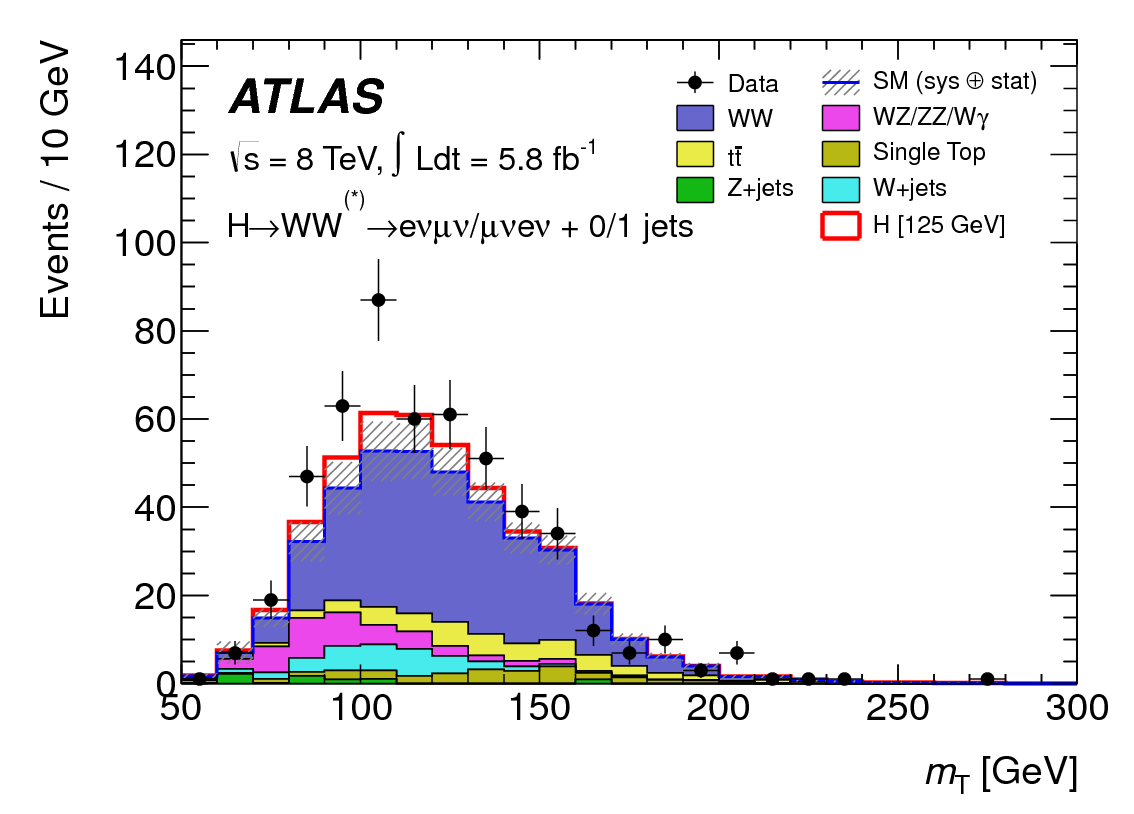
\includegraphics[width=0.6\textwidth]{figures/discovery_mt}
  \caption{$\mT$ distribution in the $H\to WW \to e\nu\mu\nu$ $\Njet \leq 1$ channels for $8 \TeV$ data~\cite{Discovery}.}
  \label{fig:disc_mt}
\end{figure}


\section{$H\to\gamma\gamma$ search}

The $H\to\gamma\gamma$ analysis is a search for a peaked excess above a falling SM diphoton mass spectrum, with $m_{\gamma\gamma}$ as the ultimate discriminating variable\footnote{The ultimate shape of the SM $\gamma\gamma$ mass spectrum depends on the requirements used to define the signal region in the analysis.}. Events are selected by requiring two isolated photons, with the leading (sub-leading) photon required to have $E_{T} > 40 (30) \GeV$. In the $8 \TeV$ data, the photons are required to pass identification criteria consistent with a photonic shower in the electromagnetic calorimeter and little leakage in the hadronic calorimeter. 

The main challenges for this analysis are accurate mass reconstruction and $m_{\gamma\gamma}$ background shape estimation. In order to accurately reconstruct the invariant mass of the di-photon system, both the energy and direction of the photons must be measured well. Therefore, the identification of the primary vertex of the hard interaction is particularly important, and is done using a multivariate likelihood which combines information about the photon direction and vertex position. The background is modeled with a falling spectrum in $m_{\gamma\gamma}$ that is parameterized by different functions depending on the category of the event.

The resulting diphoton mass spectrum is shown in figure~\ref{fig:disc_mgg}. The best fit mass value in the $\gamma\gamma$ channel alone in the combined $7$ and $8 \TeV$ data is $126.5 \GeV$. The local significance as this mass value is $4.5\sigma$, with an expected significance of $2.5\sigma$. Therefore, the measured signal strength $\mu$ is $1.8 \pm 0.5$ in this channel. 

\begin{figure}[h!]
  %\vspace{20pt}
  \centering
  \captionsetup{justification=centering}
  %\hspace*{-32pt}
  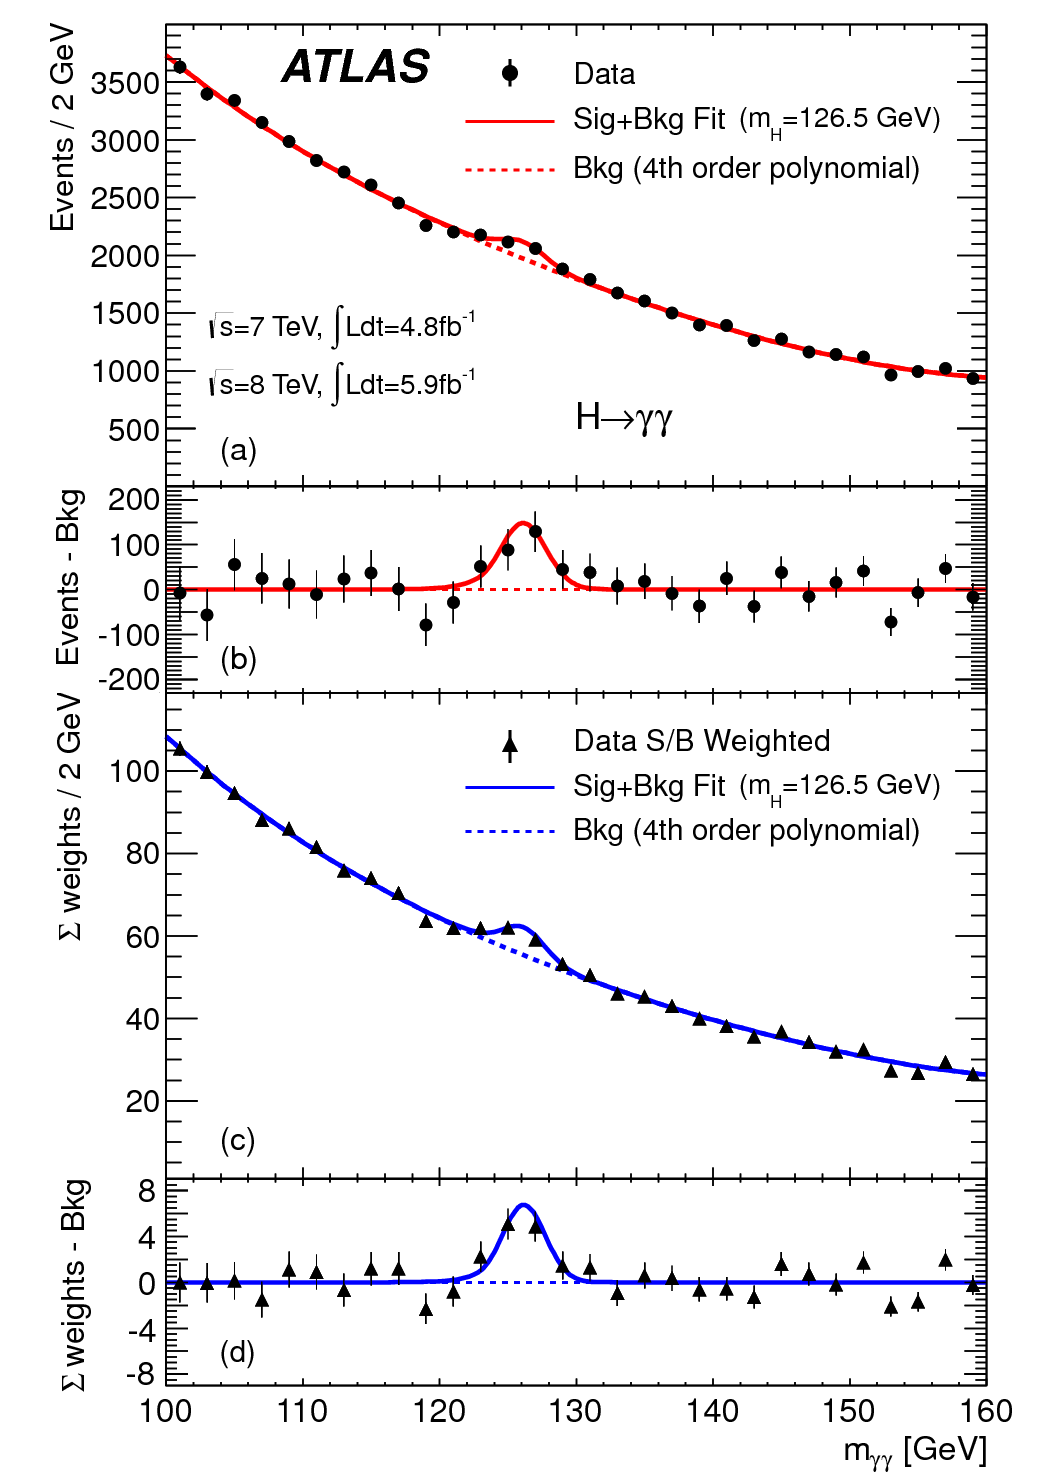
\includegraphics[width=0.5\textwidth]{figures/discovery_mgg}
  \caption{Diphoton mass spectrum in $7$ and $8 \TeV$ data. Panel a) shows the unweighted data distribution superimposed on the background fit, while panel c) shows the data where each event category is weighted by its signal to background ratio. Panels b) and d) show the respective distributions with background subtracted~\cite{Discovery}.}
  \label{fig:disc_mgg}
\end{figure}

\section{$H\to ZZ \to 4\ell$ search}

The $H\to ZZ \to 4\ell$ analysis searches for a Standard Model Higgs boson decaying to two $Z$ bosons, each of which decays to a pair of same flavor, opposite charge isolated leptons. The ultimate discriminating variable is $m_{4\ell}$, or the invariant mass of the four selected leptons. The $\ell$ denotes an $e$ or $\mu$ as with the \HWWfull analysis. Four distinct signal regions are constructed depending on the flavors of the final state, additionally separated by the flavor of the leading lepton pair. These are referred to as $4e$, $2e2\mu$, $2\mu2e$, $4\mu$. 

The main backgrounds in the $H\to ZZ \to 4\ell$ search are continuum $ZZ^*$ production, $Z$+ jets production, and $\ttbar$. The $m_{4\ell}$ distribution for background is estimated from simulation. The normalization of the SM $ZZ^*$ background is also taken from MC simulation, while the $Z$+jets and $\ttbar$ normalizations are taken from data-driven methods.

Figure~\ref{fig:disc_zz_result} shows the $m_{4\ell}$ spectrum measured in the $7$ and $8 \TeV$ datasets. There are $13$ total events observed in the window between $120$ and $130 \GeV$, with $6$ events in the $4\mu$ channel, $2$ events in the $4e$ channel, and $5$ events in the $2e2\mu/2\mu2e$. The best fit $\mu$ value in the combined $7$ and $8 \TeV$ data occurs at $125 \GeV$ and is measured to be $1.2 \pm 0.6$. The observed significance at this mass is $3.6\sigma$, with an expected significance of $2.7\sigma$. 

\begin{figure}[h!]
  %\vspace{20pt}
  \centering
  \captionsetup{justification=centering}
  %\hspace*{-32pt}
  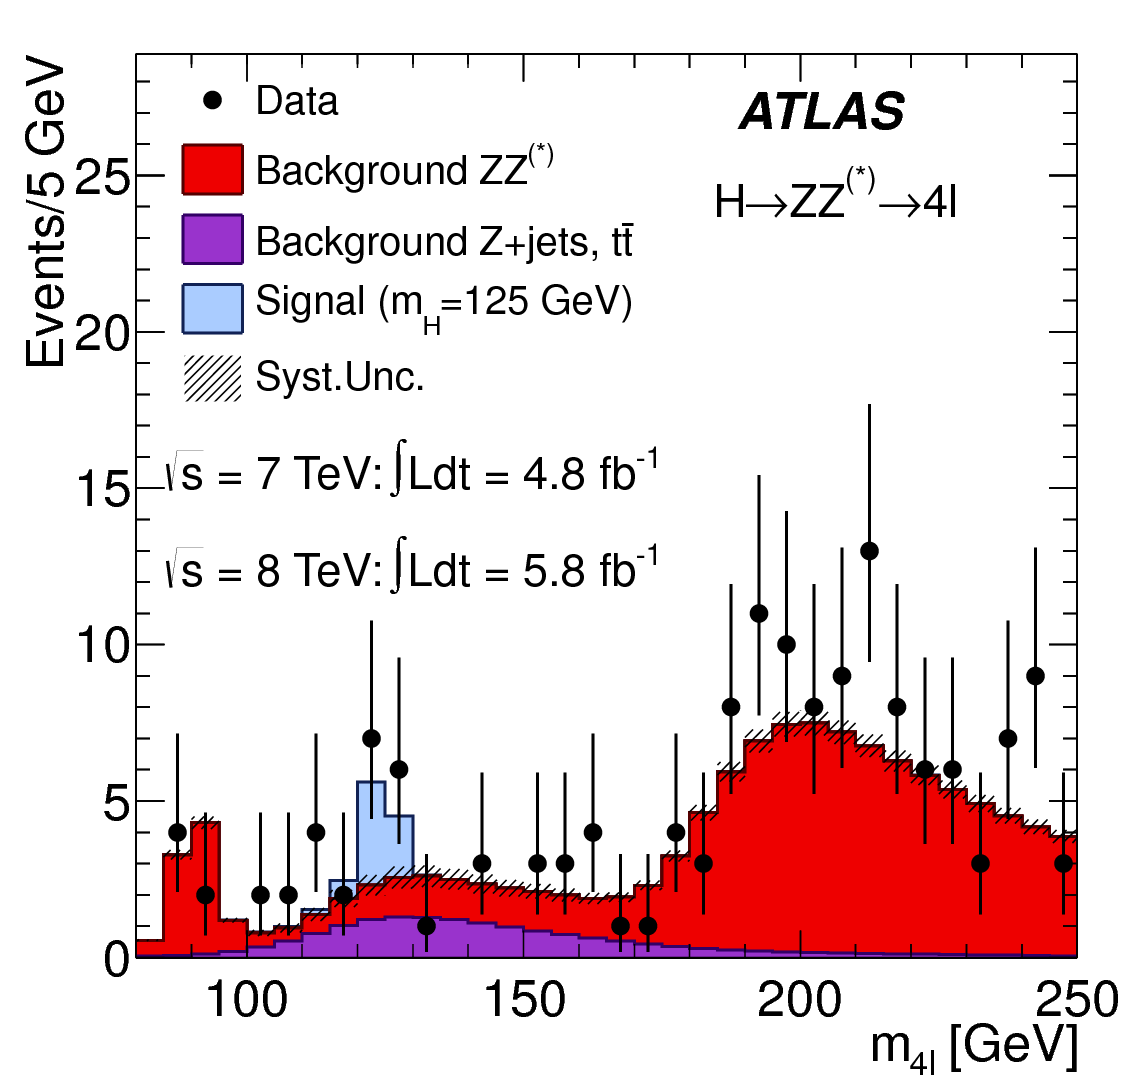
\includegraphics[width=0.6\textwidth]{figures/discovery_m4l}
  \caption{Four lepton invariant mass spectrum ($m_{4\ell}$) in $7$ and $8 \TeV$ data compared to background estimate. A $125 \GeV$ SM Higgs signal is shown in blue~\cite{Discovery}.}
  \label{fig:disc_zz_result}
\end{figure}

\section{Combined results}

The statistical interpretation of the combined results is undertaken as described in section~\ref{sec:ww_stats}, with a hypothesis test based on a likelihood ratio parameterized by the Higgs signal strength $\mu$. The null hypothesis corresponds to $\mu = 0$, while the SM Higgs corresponds to $\mu = 1$. 

\begin{table}[h!]
\centering
\captionsetup{justification=centering}

%\begin{tabular*}{0.480\textwidth}{p{0.075\textwidth} p{0.180\textwidth} l}
\hspace{-10pt}
\begin{tabular}{|c|c|c|c|c|}
\hline
Channel & Fit var. & Observed $Z_l$ & Expected $Z_l$ & $\hat{\mu}$ \\ \hline
$H\to ZZ^* \to 4\ell$ & $m_{4\ell}$ & $3.6$ & $2.7$ & $1.2 \pm 0.6$ \\ \hline
$H\to\gamma\gamma$ & $m_{\gamma\gamma}$ & $4.5$ & $2.5$ & $1.8 \pm 0.5$ \\ \hline
$H\to WW^* \to e\nu\mu\nu$ & $\mT$ & $2.8$ & $2.3$ & $1.3 \pm 0.5$ \\ \hline
Combined & - & $6.0$ & $4.9$ & $1.4 \pm 0.3$ \\ \hline
\end{tabular}

\caption{
Summary of the expected and observed significance and measured signal strengths in the combined $7$ and $8 \TeV$ datasets for the Higgs discovery analysis~\cite{Discovery}. 
}
\label{tab:discovery_summary}
\end{table}

Table~\ref{tab:discovery_summary} summarizes the properties of the individual channels as well as the significances of the excesses seen. The most significant observed local excess comes from the $\gamma\gamma$ channel. Figure~\ref{fig:disc_p0_comp} shows a comparison of the observed local $p_0$ values as a function of hypothesized mass for the three different search channels. Both the $ZZ^*$ and $\gamma\gamma$ channels have very peaked excesses, while the $WW^*$ excess can be seen as very broad because the $\mT$ distribution does not provide detailed information about the true Higgs mass. Note that all three channels shown have very similar expected significances for the Higgs signal. While the $4\ell$ and $\gamma\gamma$ channels measure excesses in data larger than that expected from the SM Higgs, the \HWWfull channel is still very comparable in sensitivity. Figure~\ref{fig:discovery_combined} shows the combined exclusion limit, $p_0$, and signal strength. The highest local excess comes at a value of $126.5 \GeV$ and corresponds to a $6.0\sigma$ observed excess. 

\begin{figure}[h!]
  %\vspace{20pt}
  \centering
  \captionsetup{justification=centering}
  %\hspace*{-32pt}
  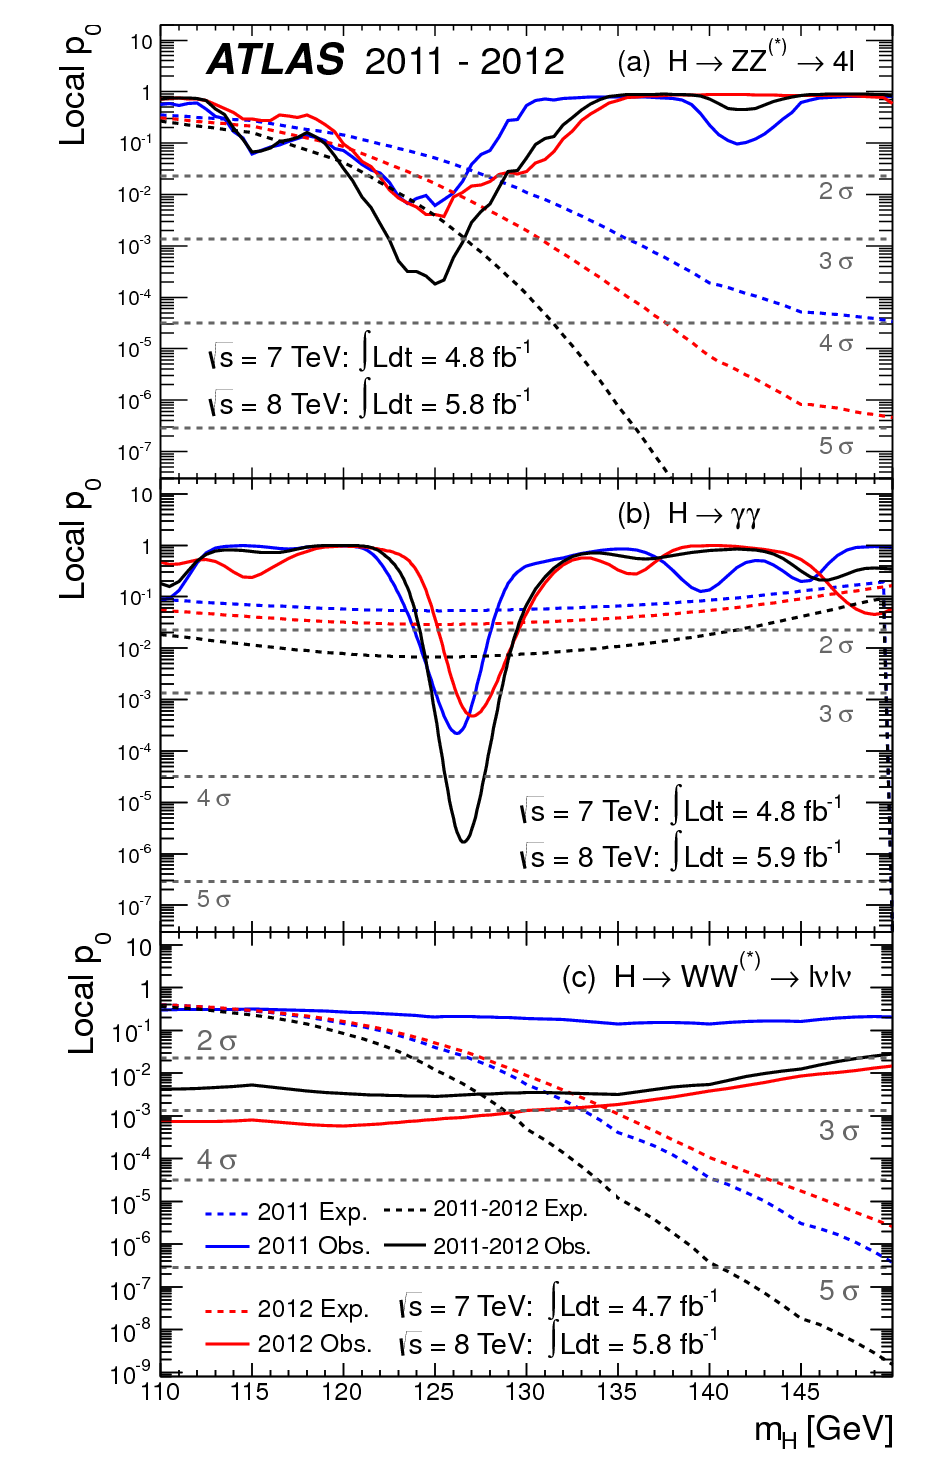
\includegraphics[width=0.6\textwidth]{figures/discovery_p0_comp}
  \caption{Local $p_0$ distribution as a function of hypothesized Higgs mass for the $H\to ZZ^* \to 4\ell$ (a), $H\to\gamma\gamma$ (b), and $H\to WW^*\to \ell\nu\ell\nu$ (c) channels. Dashed curves show expected results, while solid curves show observed. Red curves are from $7 \TeV$ data, blue curves from $8\TeV$, and black curved combined~\cite{Discovery}.}
  \label{fig:disc_p0_comp}
\end{figure}

\begin{figure}[h!]
  %\vspace{20pt}
  \centering
  \captionsetup{justification=centering}
  %\hspace*{-32pt}
  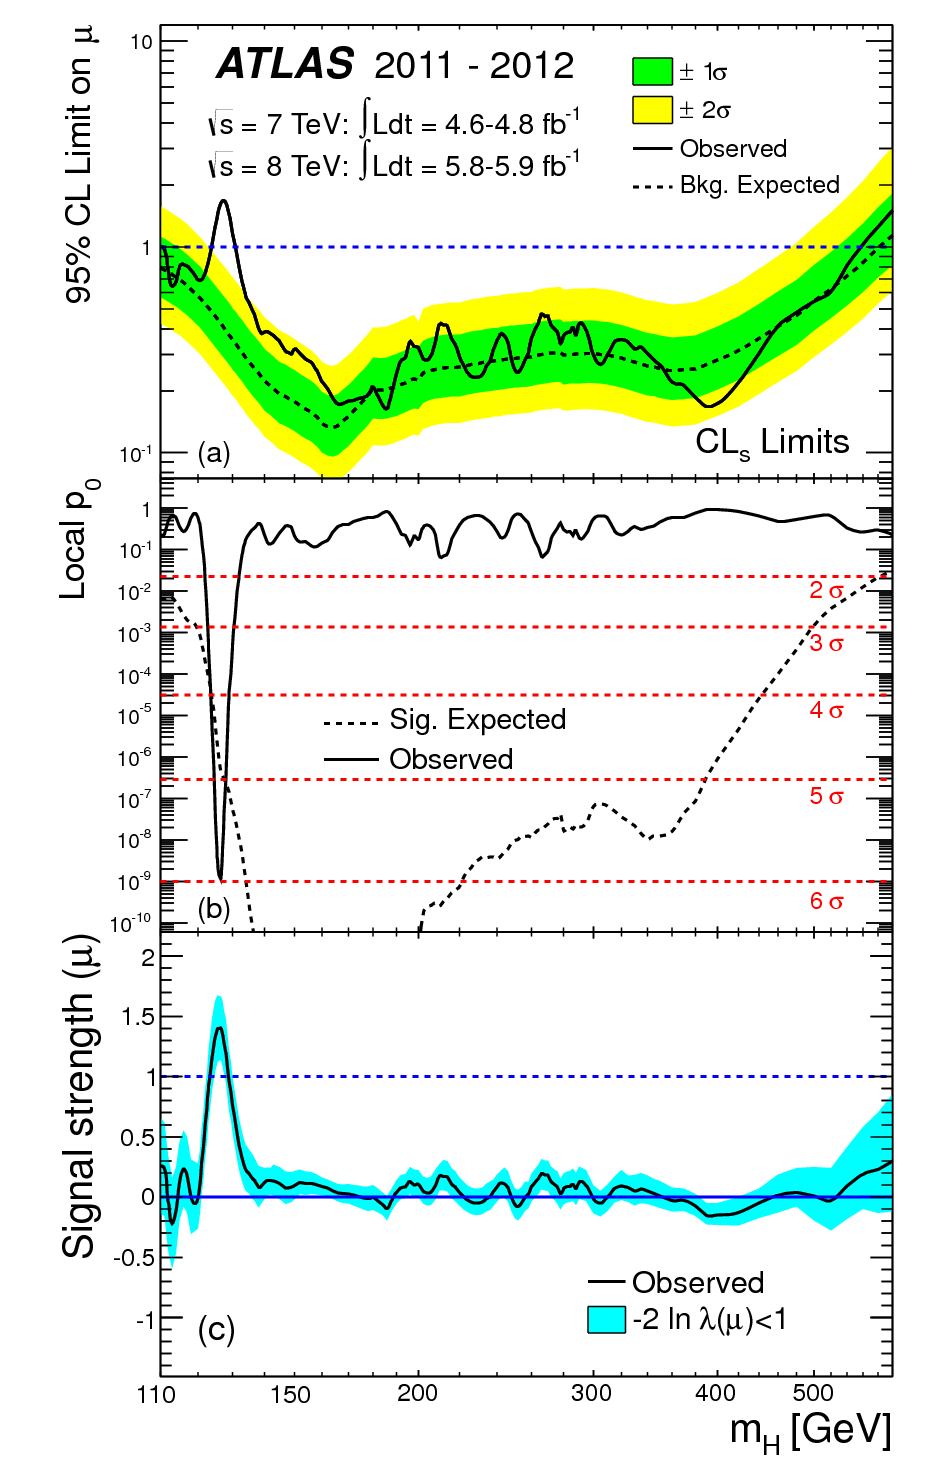
\includegraphics[width=0.6\textwidth]{figures/discovery_combined}
  \caption{Combined 95\% CL limits (a), local $p_0$ values (b), and signal strength measurement (c) as a function of Higgs mass~\cite{Discovery}.}
  \label{fig:discovery_combined}
\end{figure}

Figure~\ref{fig:discovery_mu} and table~\ref{tab:discovery_summary} show a comparison of the measured signal strengths between the different Higgs search channels. All measured $\mu$ are consistent with unity within their uncertainty, and the combined $\mu$ measurement is $1.4 \pm 0.3$. This indicates that the observed Higgs is consistent with the expectation from a SM Higgs in this dataset.  

\begin{figure}[h!]
  %\vspace{20pt}
  \centering
  \captionsetup{justification=centering}
  %\hspace*{-32pt}
  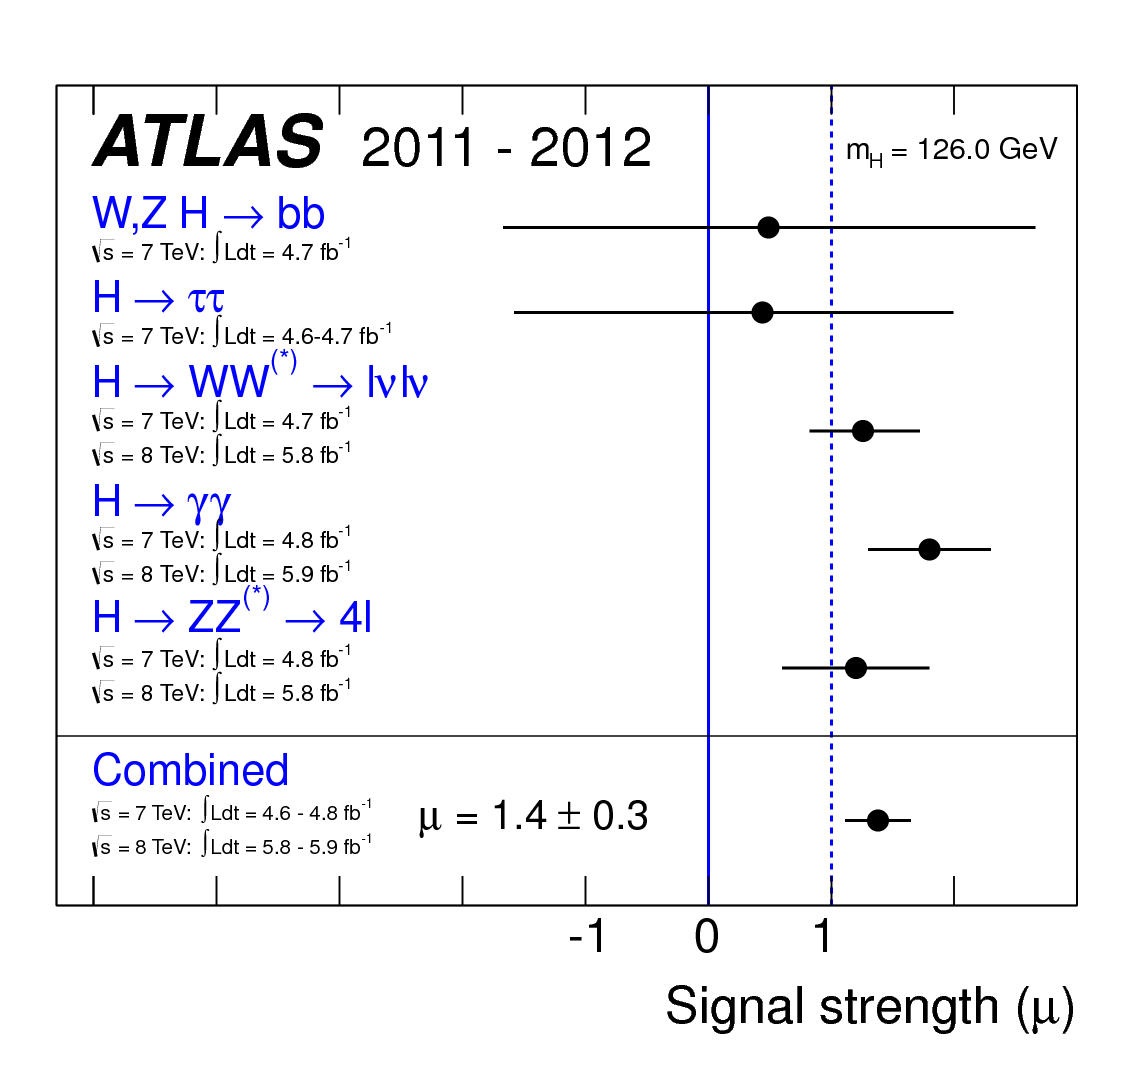
\includegraphics[width=0.6\textwidth]{figures/discovery_mu}
  \caption{Comparison of measured signal strength $\mu$ for a $126 \GeV$ Higgs in the $7$ and $8 \TeV$ datasets~\cite{Discovery}.}
  \label{fig:discovery_mu}
\end{figure}

The likelihood can also be computed in a two-dimensional plane of $m_{H}$ and $\mu$, and this is shown in figure~\ref{fig:disc_2d}. The results show that while the $\gamma\gamma$ and $ZZ^*$ channels have very good mass resolution, the excess in $WW^*$ covers a broad mass range. The banana shape of the $WW^*$ result is due to the fact that the excess in this channel can either be explained by increasing the signal strength or by changing the mass (and thus the cross section). The two parameters are correlated due to the lack of mass sensitivity in this channel. 

\begin{figure}[h!]
  %\vspace{20pt}
  \centering
  \captionsetup{justification=centering}
  %\hspace*{-32pt}
  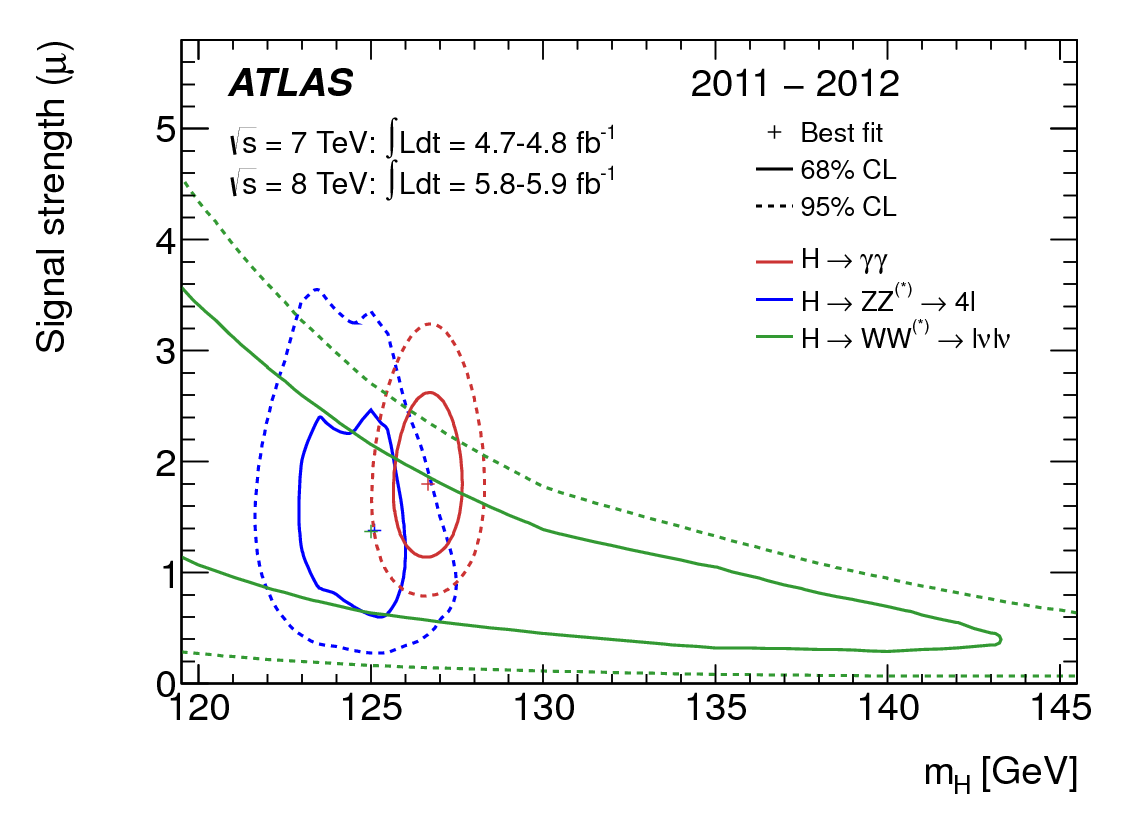
\includegraphics[width=0.6\textwidth]{figures/disc_2d}
  \caption{Two dimensional likelihood as a function of signal strength $\mu$ and Higgs mass $m_H$~\cite{Discovery}.}
  \label{fig:disc_2d}
\end{figure}

Because multiple Higgs mass points are searched for, the local significance must be corrected for a look-elsewhere effect to compute a true global significance. The global significance for finding a Higgs anywhere in the mass range of $110 \GeV$ to $600 \GeV$ is $5.1\sigma$. This increases slightly to $5.3\sigma$ if only mass range from $110$ to $150 \GeV$ are considered. 

\section{Conclusion}

A new particle consistent with the Higgs boson was observed using $4.8 \ifb$ collected at $\sqrt{s} = 7 \TeV$ and $5.8 \ifb$ at $\sqrt{s} = 8 \TeV$. The measured mass of the particle is $126.5 \GeV$ with a global (local) significance of $5.1 (6.0)\sigma$. This discovery was achieved using the \HWWfull, $H\to\gamma\gamma$, and $H\to ZZ\to 4\ell$ channels. All three of these channels had very similar expected significances for observing the SM Higgs ($2.3$-$2.7\sigma$ in each channel). Even with worse mass resolution, the $WW^*$ channel contributed to the expected sensitivity due to the large branching ratio of the Higgs to this final state. The observed significances were $2.8\sigma$ in the $WW^*$ channel, $3.6\sigma$ in the $ZZ^*$ channel , and $4.5\sigma$ in the $\gamma\gamma$ channel. This result is the first discovery level observation of a particle consistent with the Higgs. 

